\section{Módulos del sistema}
	Durante este Trabajo Terminal  se han desarrollado los módulos de:
	\begin{itemize}
		\item \textbf{Profesores}
		\item \textbf{Salones}
	\end{itemize}
Los cuales serán explicados a continuación.
\section{Modulo de Profesores}	El módulo de \textbf{Profesores} consiste en el prototipo de una agenda de contactos con la plantilla del personal docente de la escuela, el cuál muestra el nombre, cubículo y fotografía de los profesores. Este prototipo también cuenta con detalles de medios de contacto de los profesores los cuales son:
	\begin{itemize}
		\item Cubículo
		\item Horario de Atención
		\item E-mail
		\item Teléfono
		\item Página Web
	\end{itemize}
	Así mismo se puede visualizar algunos datos que denotan la experiencia del profesor, los cuales son:
	\begin{itemize}
		\item Materias impartidas
		\item Trabajos Terminales dirigidos
	\end{itemize} 
	\subsection{Etapa de Análisis}
	Durante este módulo nos enfrentamos a distintos problemas, uno de los primeros al que nos enfrentamos fue el como obtendríamos la información, después de analizar la situación nos dimos cuenta que algunos datos de un profesor no son privados, los cubículos, el horario de atención ya que al ser miembros del personal docente de la institución se les asigna un cubículo y horarios de atención que los alumnos deben conocer. \\
	
	 Sin embargo aún se mantenía el problema de la  información confidencial, ya que la fotografía del profesor es un dato personal y  la escuela no tiene la facultad de publicar sin el consentimiento del profesor. Así que se llegó a la decisión de tener un aviso de privacidad el cuál deberá ser aceptado para subir una fotografía.\\
	 
	 El siguiente punto al que nos enfrentamos después de definir el como obtendríamos los datos fue el saber cuál o quién sería nuestra fuente de información, ya que sabíamos qué no existía algún servicio web que pudiera proporcionar los datos que ya teníamos definidos.  En primera instancia analizamos la posibilidad de que una persona fuera responsable de brindarnos la información de cada profesor, después de reuniones con nuestros sinodales y sus observaciones realizamos una reunión con nuestros directores y se tomó la decisión de delegar esta tarea a cada profesor.\\
	 
	 Después e realizo la tarea del diseño de las interfaces de usuario del alumno las cuales fueron desarrolladas con ayuda del software "Balsamiq Mockups" y se muestran en las figuras: \ref{fig:maquetaprofesor} y \ref{fig:maquetaprofesorSeleccionado}
	 \begin{figure}[h!]
	 	\begin{center}
	 		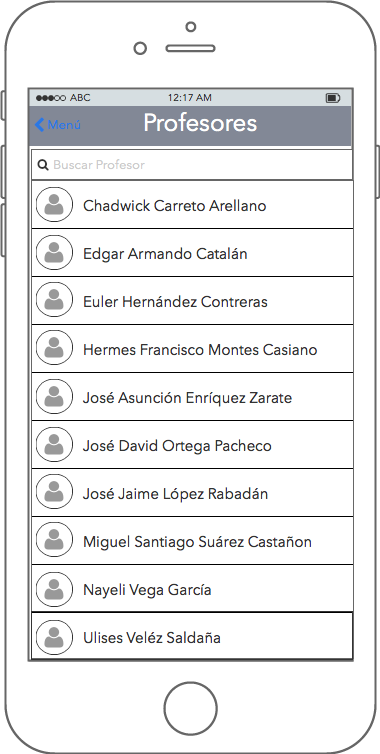
\includegraphics[width=0.3\textwidth]{images/maqueta/UIP4Profesores.png}
	 		\caption{Maqueta IUP4 Profesores.}
	 		\label{fig:maquetaprofesor}
	 	\end{center}
	 \end{figure}
 \begin{figure}[h!]
 	\begin{center}
 		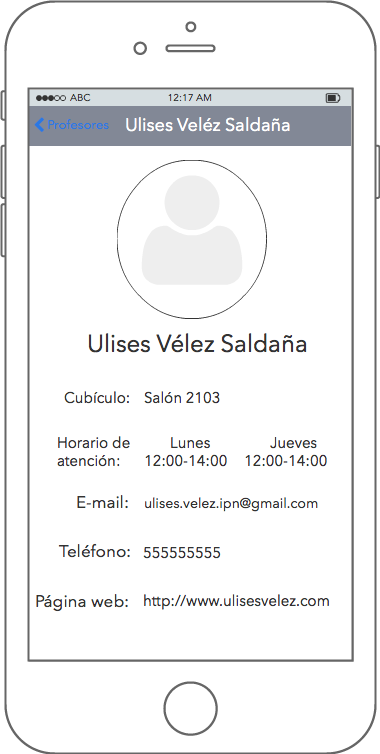
\includegraphics[width=0.3\textwidth]{images/maqueta/UIP41ProfesorSeleccionado.png}
 		\caption{Maqueta IUP4.1 Profesor Seleccionado.}
 		\label{fig:maquetaprofesorSeleccionado}
 	\end{center}
 \end{figure}
	\subsection{Etapa de Desarrollo }
	 
	 El desarrollo de la aplicación está basado en \textit{Programación Orientado a Objetos} lo cual nos permite realizar los principios de abstracción, herencia, polimorfismo y encapsulamiento. Una vez comprendido los principios mencionados anteriormente nos dimos a la tarea de crear al objeto \textit{Profesor} y sus atributos. \\
	 
	  Para realizar la etapa del desarrollo de este modulo concebimos algunas pruebas de concepto, esto con la finalidad de ver si era posible desarrollar con la tecnología seleccionada  lo analizado anteriormente, para esta tarea tuvimos que realizar una investigación sobre como crear vistas en tablas en el lenguaje \textbf{Swift}.\\
	  
	  Al realizar la investigación pudimos entender el uso de las tablas dentro de un dispositivo móvil, esto se puede realizar gracias a los componentes \textbf{'Table View '} y \textbf{'Custom Cell View' } y  a sus respectivas clases \textbf{'TableViewController'}, \textbf{'TableViewDelegate'} y \textbf{ 'CellViewController'}. \\
	  
	  Una vez comprendido el comportamiento de estos componentes y las clases  que los delegan dio inicio la etapa de implementación del componente en nuestro prototipo del módulo de profesor. A continuación se muestran algunas evidencias de los códigos que fueron implementados para este módulo en las figuras: \ref{profesorc}, \ref{tableC}, \ref{tableCC}\\
	 
	 \begin{figure}[h!]
	 	\begin{center}
	 		\fbox{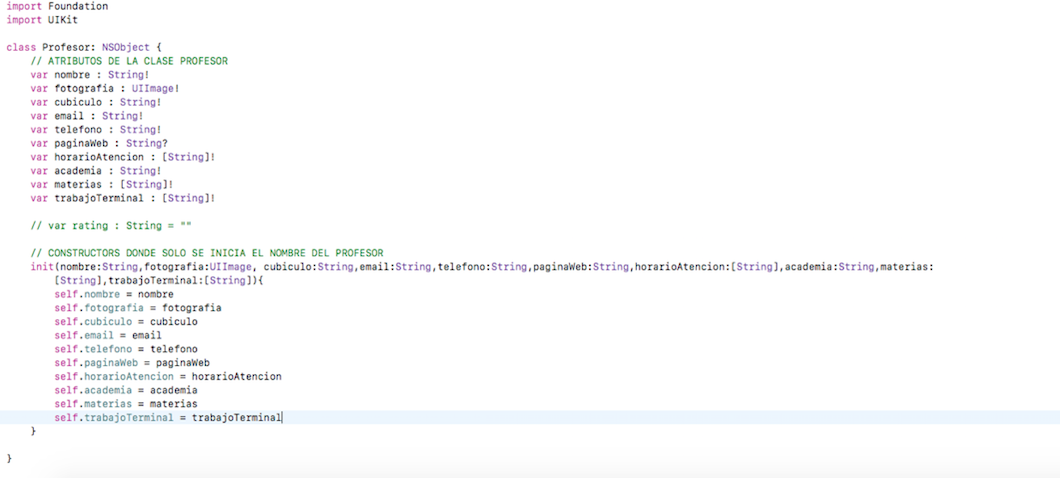
\includegraphics[width=\textwidth]{images/codigos/objetoprofesor}}	
	 		\caption{Creación Objeto Profesor.}
	 		\label{profesorc}
	 	\end{center}
	 \end{figure}
	 	 \begin{figure}[h!]
	 	\begin{center}
	 		\fbox{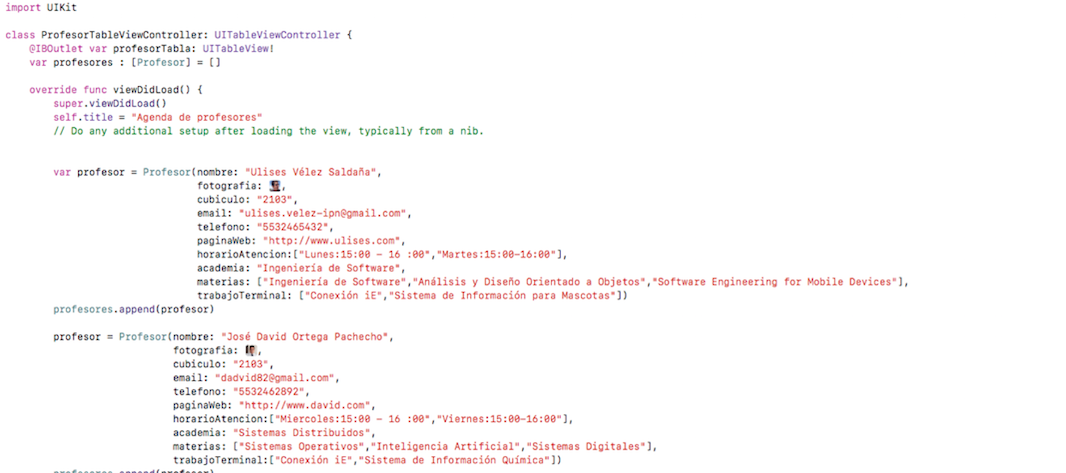
\includegraphics[width=\textwidth]{images/codigos/tableviewcontroller}}	
	 		\caption{Implementación Table View Controller.}
	 		\label{tableC}
	 	\end{center}
	 \end{figure}
 
	 \begin{figure}[h!]
	\begin{center}
		\fbox{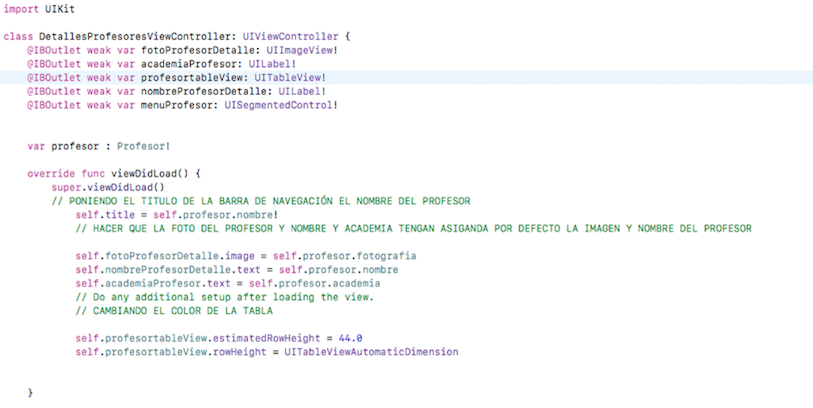
\includegraphics[width=\textwidth]{images/codigos/profesorseleccionado1}}
		\caption{Implementación Table View Cell.}
		\label{tableCC}
	\end{center}
\end{figure}

Al finalizar la etapa de desarrollo se logro obtener el prototipo de los profesores con las funcionalidades antes mencionadas como se muestra en las figuras \ref{p1}, \ref{p2} y \ref{p3}
\begin{figure}[h!]
	\begin{center}
		\fbox{\includegraphics[width=0.3\textwidth]{images/resultados/p1}}
		\caption{Agenda de Profesores.}
		\label{p1}
	\end{center}
\end{figure}

\begin{figure}[h!]
	\begin{center}
		\fbox{\includegraphics[width=0.3\textwidth]{images/resultados/p2}}
		\caption{Medios de Contacto de Profesor Seleccionado .}
		\label{p3}
	\end{center}
\end{figure}

\begin{figure}[h!]
	\begin{center}
		\fbox{\includegraphics[width=0.3\textwidth]{images/resultados/p3}}
		\caption{Experiencia de Profesor Seleccionado.}
		\label{p2}
	\end{center}
\end{figure}

\section{Modulo de Salones}
El módulo de \textbf{Salones} consiste en el prototipo de ubicación de los salones asignados a los grupos, en el cual se puede visualizar una lista de los grupos y el salón que tiene asignado, una vez seleccionado grupo se muestra la siguiente información:
\begin{itemize}
	\item Ubicación geográfica del usuario y del edificio al que pertenece el grupo seleccionado.
	\item Mapa geográfico y marcador que indica el nombre del edificio
	\item Nivel y salón que pertenece el grupo seleccionado.
\end{itemize}  
Así como un apartado de detalles del edificio que muestra la siguiente información:
\begin{itemize}
	\item Nombre del edificio seleccionado.
	\item ID del edificio seleccionado.
	\item Niveles del edificio seleccionado
	\item Accesibilidad del edificio seleccionado.
	\item Tipos de aula que tiene el edificio seleccionado.
\end{itemize}
\subsection{Etapa de Análisis}
Al empezar la etapa de este módulo se pensaba que el análisis de este sería mucho más sencillo que el del módulo que ya teníamos realizado, pero al paso de los días nos dimos cuenta que estábamos en un completo error. Ya que al empezar a analizar mas a fondo la problemática nos dimos cuenta que sería un módulo muy complejo.\\

Como primera parte para que el alumno pudiera identificar el salón al que había sido asignado su grupo debíamos obtener esta información del área de prefectura de la escuela, al ya saber de donde obtendríamos la información de la asignación de salones comenzamos a analizar como se mostraría los datos antes mencionados.\\

En primera instancia pensamos en colocar imágenes aéreas de los edificios de la escuela, pero analizando esa posibilidad nos dimos cuenta que no era posible saber el nivel al que pertenecía el salón, si bien nos cubría la necesidad de los edificios nos generaba otros conflictos que teníamos que solventar. Así que diseñamos una vista 3D para la realización de los edificios y una vista era del nivel para saber en que lugar se encontraba el edificio.\\

Siguiendo con este análisis nos dimos cuenta que ya cubríamos la problemática que habíamos decidido atacar, pero no la cubríamos de manera satisfactoria puesto que esta propuesta de solución era muy poco funcional pues no era una vista dinámica.\\

Así que nos propusimos a rediseñar nuestra propuesta de solución, en esta nueva propuesta se mantuvo la vista 3D del edificio y la vista aérea del nivel pero con la diferencia que está vez decidimos utilizar mapas geográficos y y la ubicación geográfica del alumno. Esto con la finalidad de darle una mejor ubicación de la escuela al alumno, con esta vista podría ver que tan cerca o que tan lejos se encuentra del edificio, así como poder girar los mapas de norte a sur y de este a oeste para una mejor localización, así como implementar un acercamiento sobre los mapas y ver un poco mas detallado el área en donde se encuentra. Ademas de brindarle detalles sobre el edificio como el tipo de aulas que tiene el edificio, la accesibilidad al edificio así como los servicios con los que cuenta.\\

Una vez definida nuestra propuesta de solución decdimos realizar la maqueta que se muestra en las figuras \ref{fig:maquetasalon1}, \ref{fig:maquetasalon2}, \ref{fig:maquetasalon3} y \ref{fig:maquetasalon4},   
 \begin{figure}[h!]
	\begin{center}
		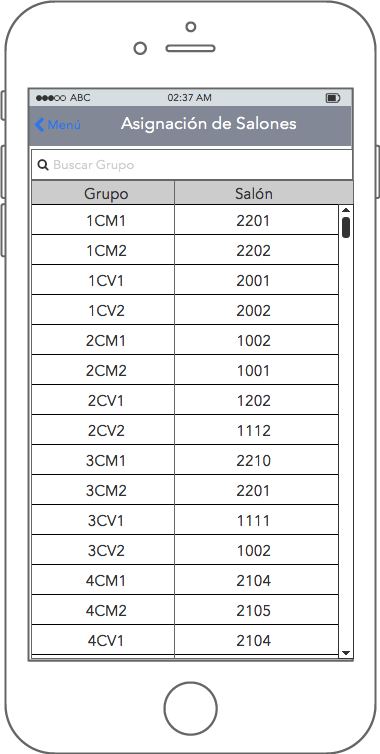
\includegraphics[width=0.3\textwidth]{images/maqueta/UIS3AsignaciondeSalones.png}
		\caption{Maqueta IUS3 Asignación de Salones.}
		\label{fig:maquetasalon1}
	\end{center}
\end{figure}
 \begin{figure}[h!]
	\begin{center}
		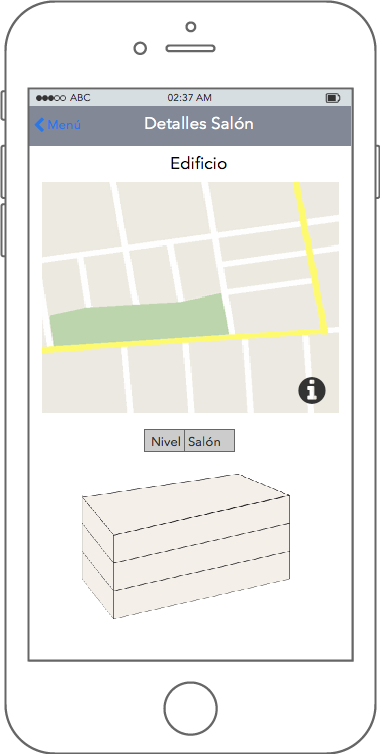
\includegraphics[width=0.3\textwidth]{images/maqueta/UIS31DetallesSalon.png}
		\caption{Maqueta IUS3.1 Detalles de Nivel.}
		\label{fig:maquetasalon2}
	\end{center}
\end{figure}
 \begin{figure}[h!]
	\begin{center}
		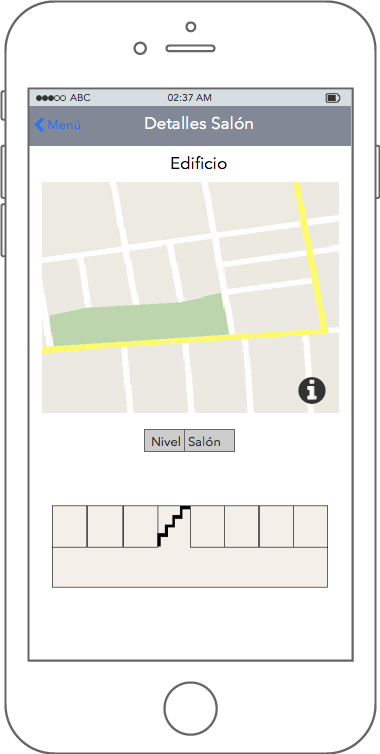
\includegraphics[width=0.3\textwidth]{images/maqueta/UIS32DetallesSalon.png}
		\caption{Maqueta IUS3.2 Detalles de Salón.}
		\label{fig:maquetasalon3}
	\end{center}
\end{figure}
 \begin{figure}[h!]
	\begin{center}
		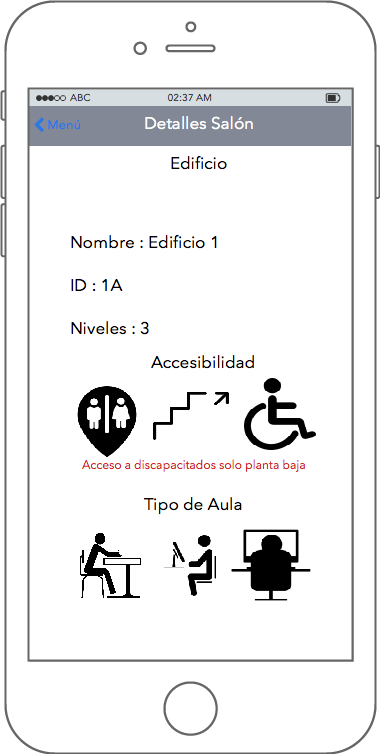
\includegraphics[width=0.3\textwidth]{images/maqueta/UIS32DetallesEdificio.png}
		\caption{Maqueta IUS3.3 Detalles de Edificio.}
		\label{fig:maquetasalon4}
	\end{center}
\end{figure}

\subsection{Etapa de Desarrollo}
Continuando con nuestra etapa de desarrollo basada en \textit{Programación Orientada a Objetos} nos dimos a la tarea de realizar la creación de nuestro objeto Salón y nuestro objeto edificio.

La parte más complicada de esta etapa fue la curva de aprendizaje de los mapas geográficos ya que encontramos tres principales herramientas que nos brindaban la solución propuesta en el análisis. Las tres principales herramientas se describen a continuación: 
\begin{itemize}
	\item \textbf{Mapbox}: Mapbox es la plataforma de datos de ubicación para aplicaciones móviles y web de código libre. Que proporciona  elementos básicos para agregar funciones de ubicación, como mapas, búsqueda y navegación.\\ Con está herramienta logramos la realización de los mapas de la escuela en 3D véase en \ref{mapbox}, un modelado que visualmente atrae mucho, pero el uso de API y SDK nos impidieron continuar trabajando con esta herramienta ya que nos costaba mucho tiempo el aprender esta herramienta y era muy costoso en términos de tiempo el implementarla en código a nuestro prototipo.
	
	\begin{figure}[h!]
		\begin{center}
			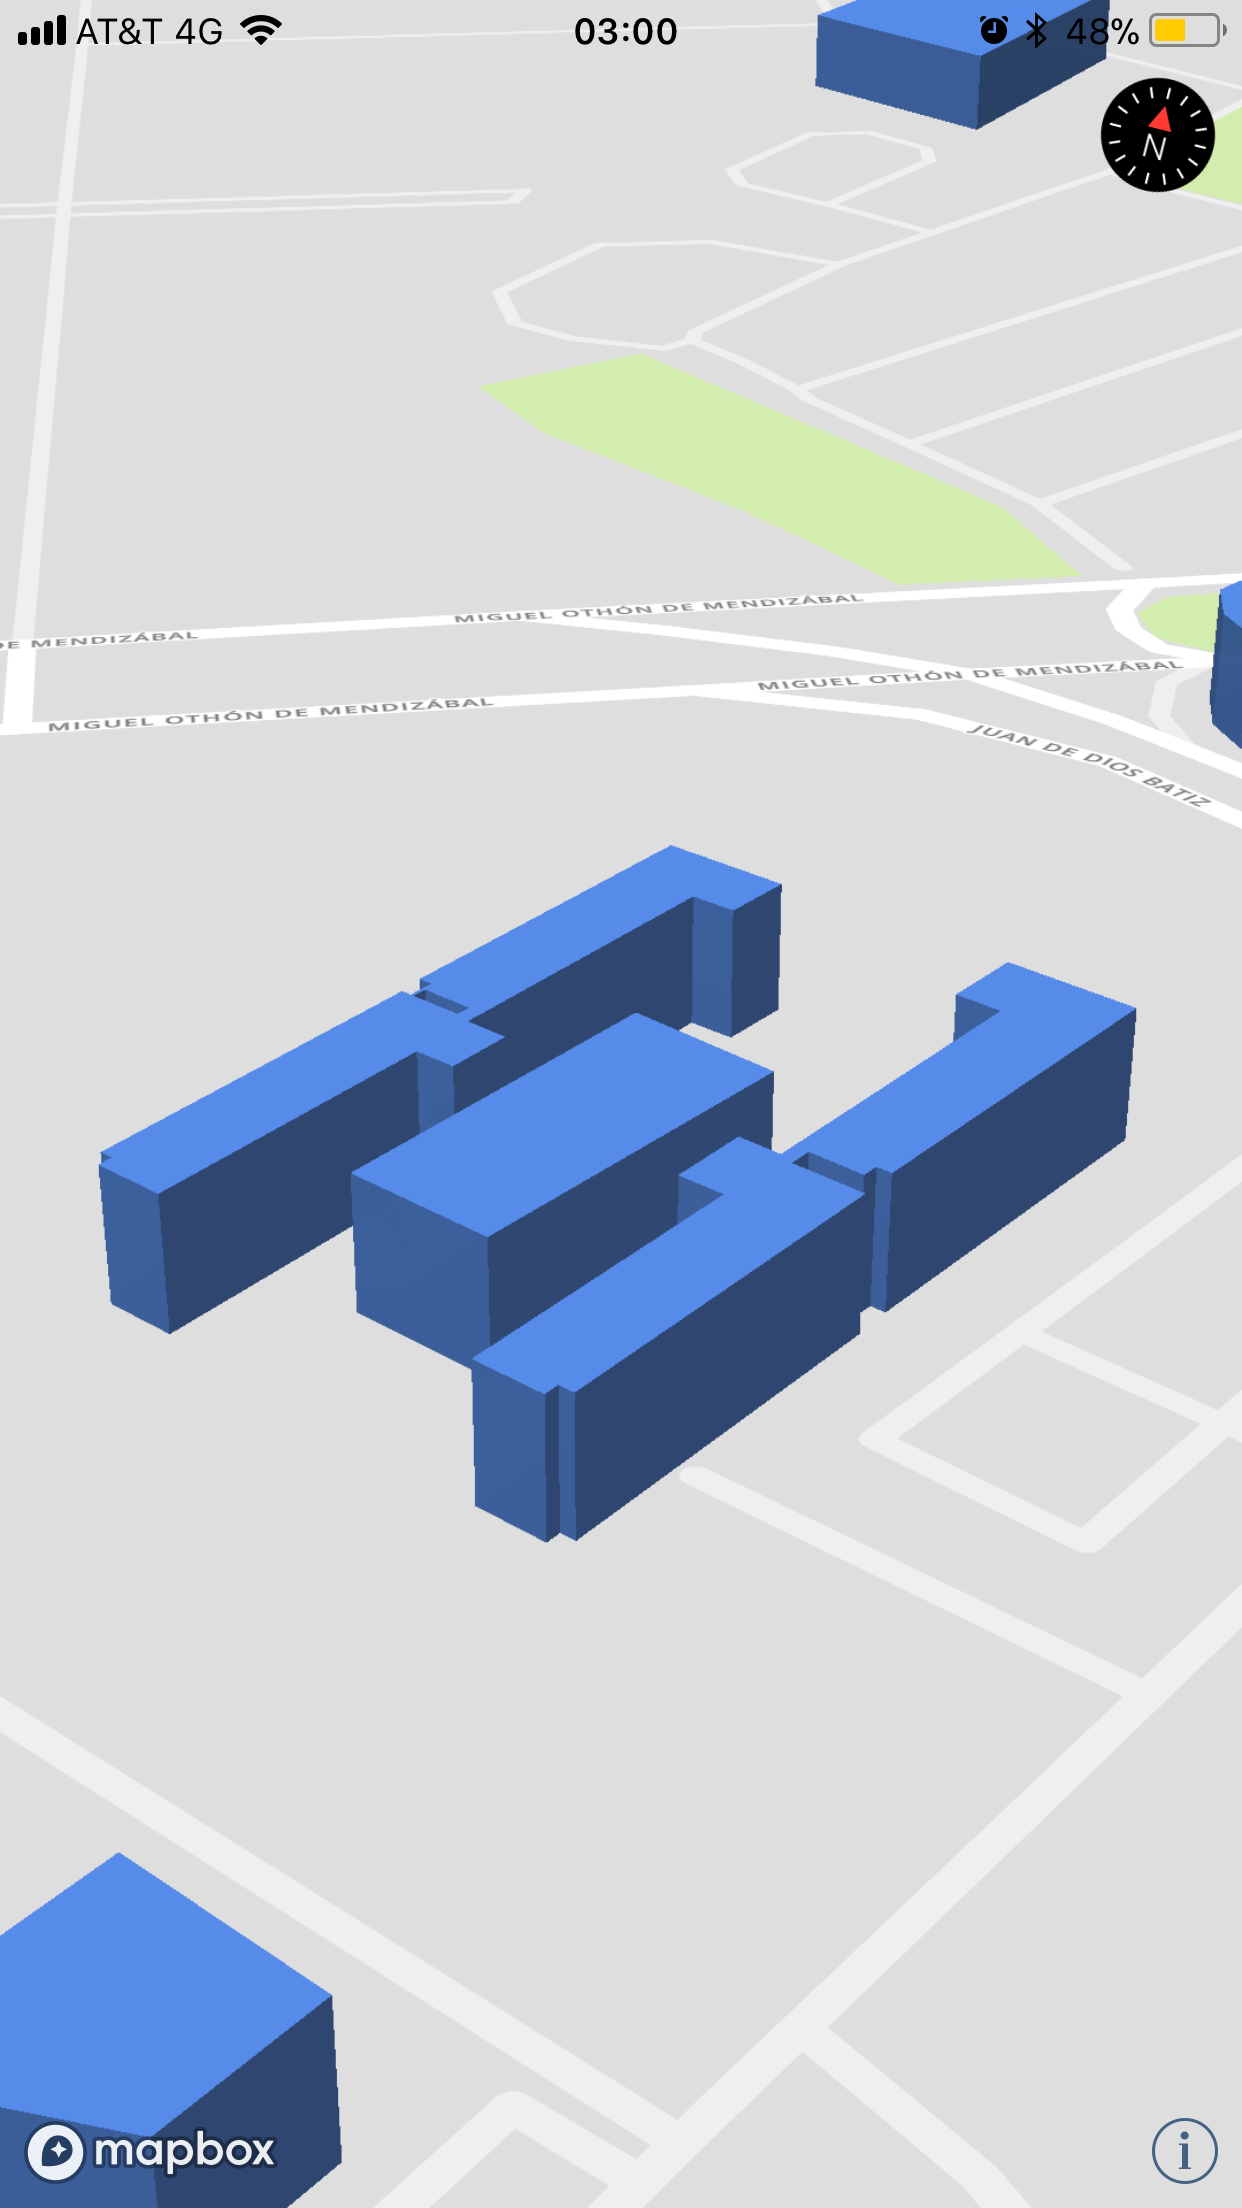
\includegraphics[width=0.3\textwidth]{images/maqueta/mapbox.png}
			\caption{Modelado 3D con Mapbox.}
			\label{mapbox}
		\end{center}
	\end{figure}
	\item  \textbf{Google Maps}: Google Maps crea aplicaciones de iOS repletas de funciones para los usuarios ya que tiene un muy amplio catalogo de funcionalidades que ayudan a hacer muy intuitivo el trato de usuario-aplicación. Sin Embargo las API's de Google Maps para iOS están disponibles a través de CocoaPods y al igual que mapbox al utilizar API's o SDK nos atrasaban en el aspecto del desarrollo pues no solo teníamos que aprender sus métodos de programación también teníamos que  aprender el uso de CocoaPods.
	\item \textbf{MapKit}: Muestra mapas o imágenes satélitales  directamente desde la interfaz de la aplicación, llama a los puntos de interés y determine la información de marcas de lugar para las coordenadas del mapa. Puede agregar anotaciones y superposiciones al mapa para llamar a puntos de interés o destinos de usuarios. Ademas de mencionar que este Framework es nativo de Apple y en su defecto funciona de manera nativa con Swift.
\end{itemize}
 Después de analizar todas las herramientas que nos podían brindar los métodos para desarrollar lo antes analizado tomamos la decisión de utilizar el framework nativo de Apple 'MapKit' ya que al no requerir de ningún API y contener una muy buena documentación de los mismos creadores del lenguaje que decidimos utilizar para el desarrollo, nos dimos a la tarea de aprender a utilizar los métodos que permitían el desarrollo de nuestras necesidades.\\
 
 Los principales  métodos y clases que nos permitieron el desarrollo de nuestro análisis fueron las siguientes: \textbf{'Mapkit'}, \textbf{'MKAnnotation'}, \textbf{'MKAnnotationView'}, \textbf{'MKPolygon'} y \textbf{'MKOverlay'}, para un mejor entendimiento del comportamiento de estas clases se desarrollo un prototipo el cual es presentado en la figura \ref{mapkit}\\
 \begin{figure}[h!]
 	\begin{center}
 		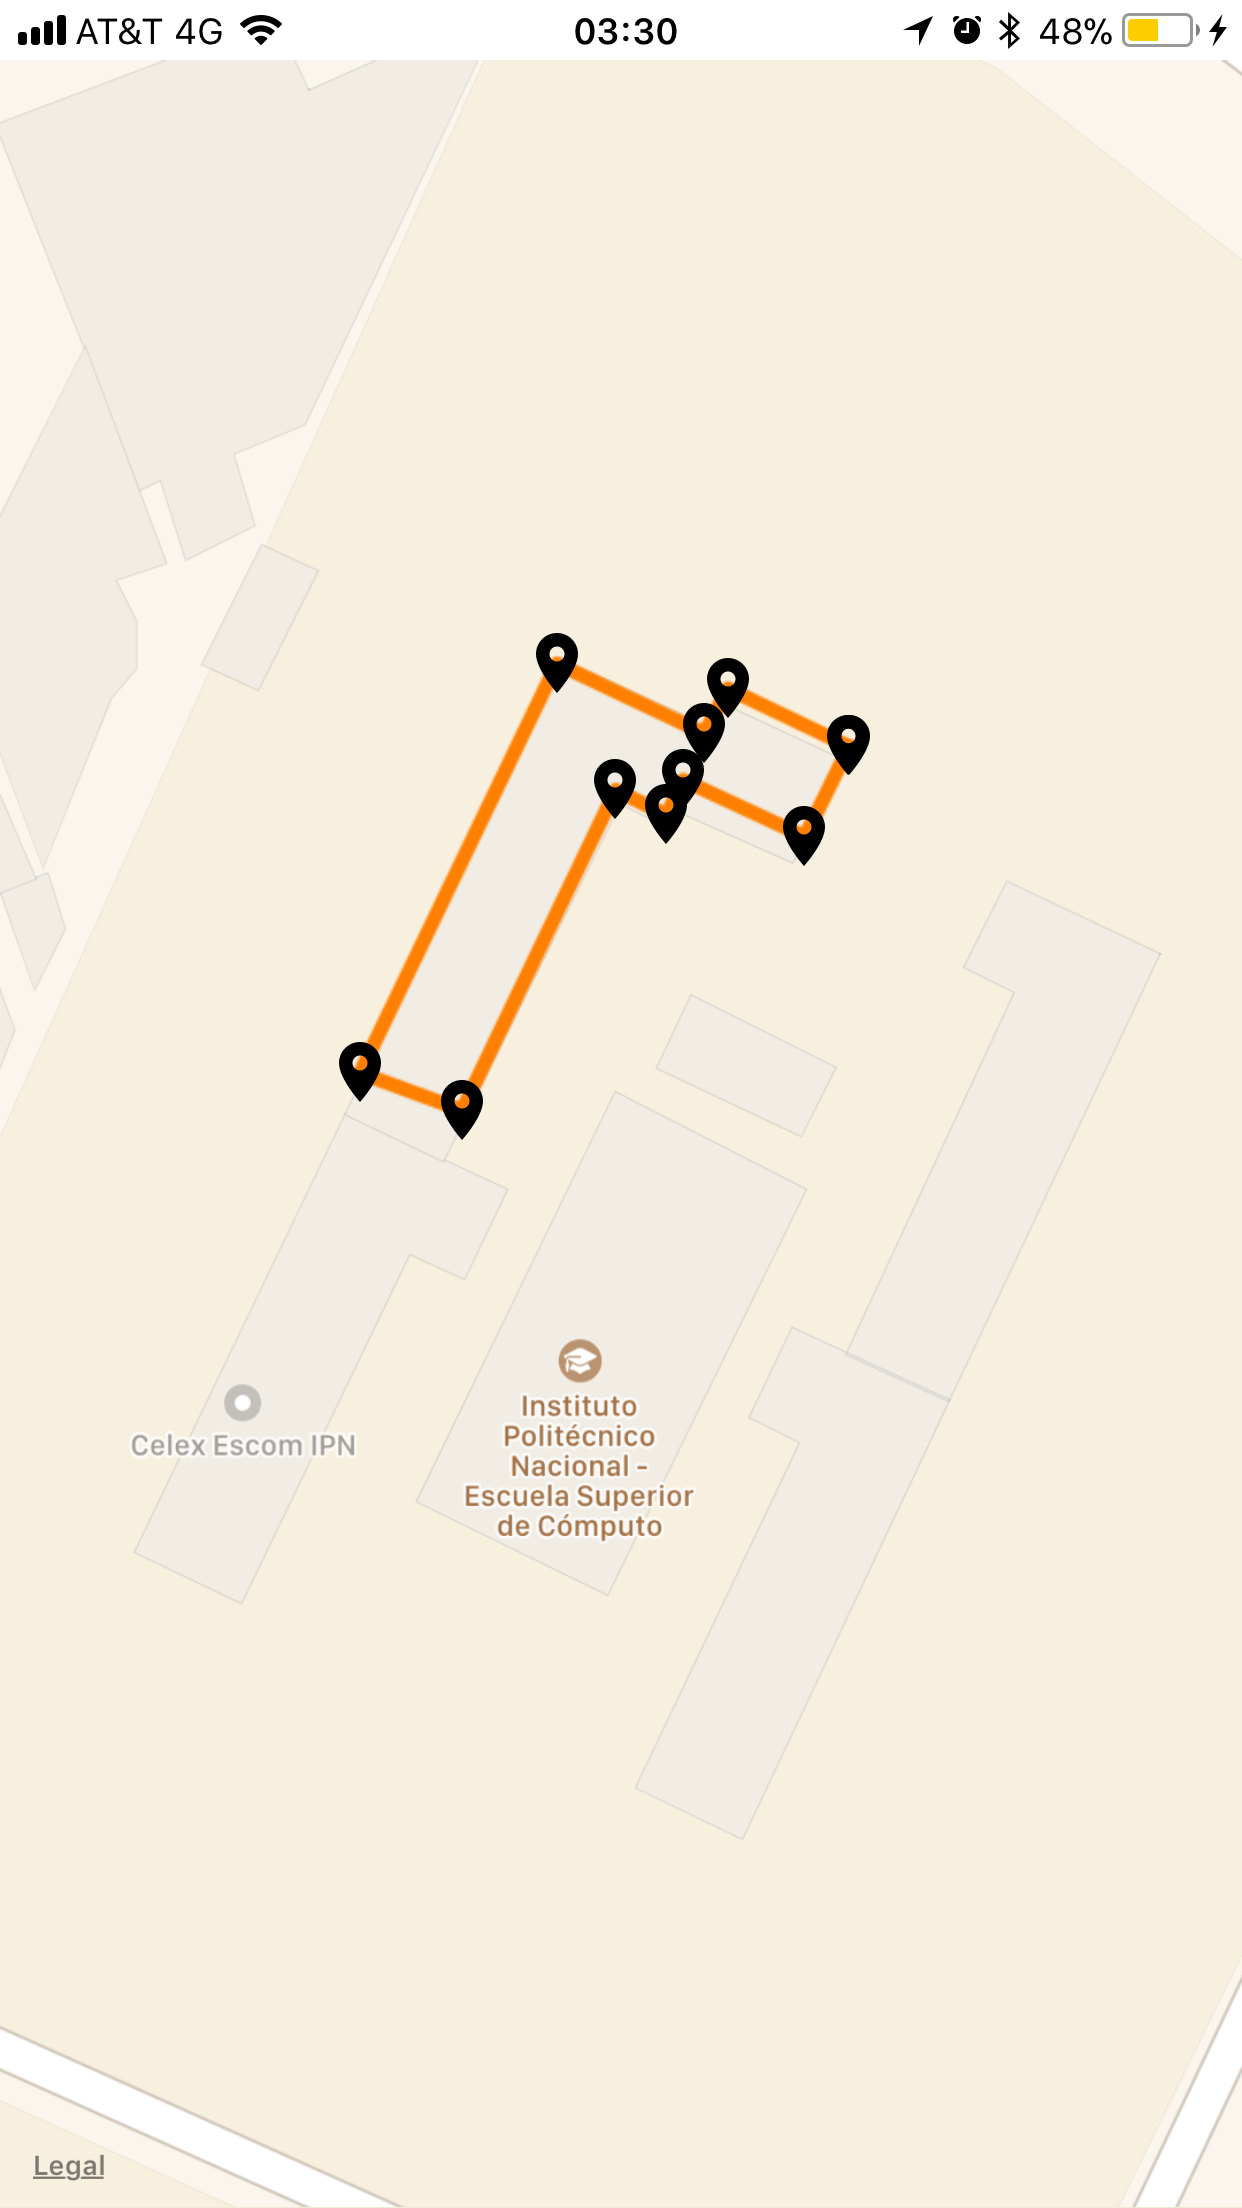
\includegraphics[width=0.3\textwidth]{images/maqueta/mapkit.png}
 		\caption{Creación de Polígonos con MapKit.}
 		\label{mapkit}
 	\end{center}
 \end{figure}

 Una vez comprendidas todas esas clases y métodos iniciamos el desarrollo del prototipo, se mostrarán algunos códigos de los fragmentos mas complejos implementados en las siguientes figuras: \ref{plist}, \ref{edificioplist}, \ref{poligono} y \ref{detalleedificio}
  \begin{figure}[h!]
 	\begin{center}
 		\fbox{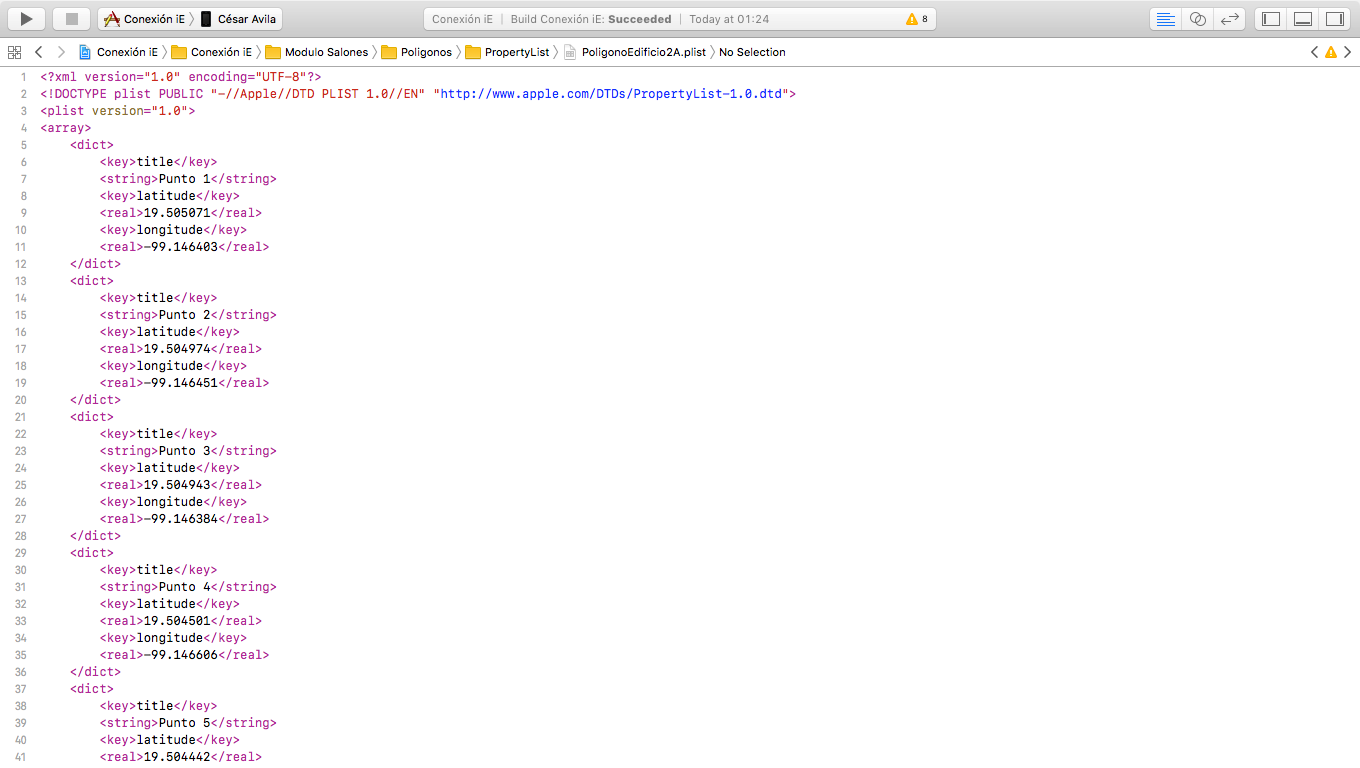
\includegraphics[width=\textwidth]{images/codigos/plist}}	
 		\caption{Creación de Property List XML de Coordenadas.}
 		\label{plist}
 	\end{center}
 \end{figure}
 \begin{figure}[h!]
	\begin{center}
		\fbox{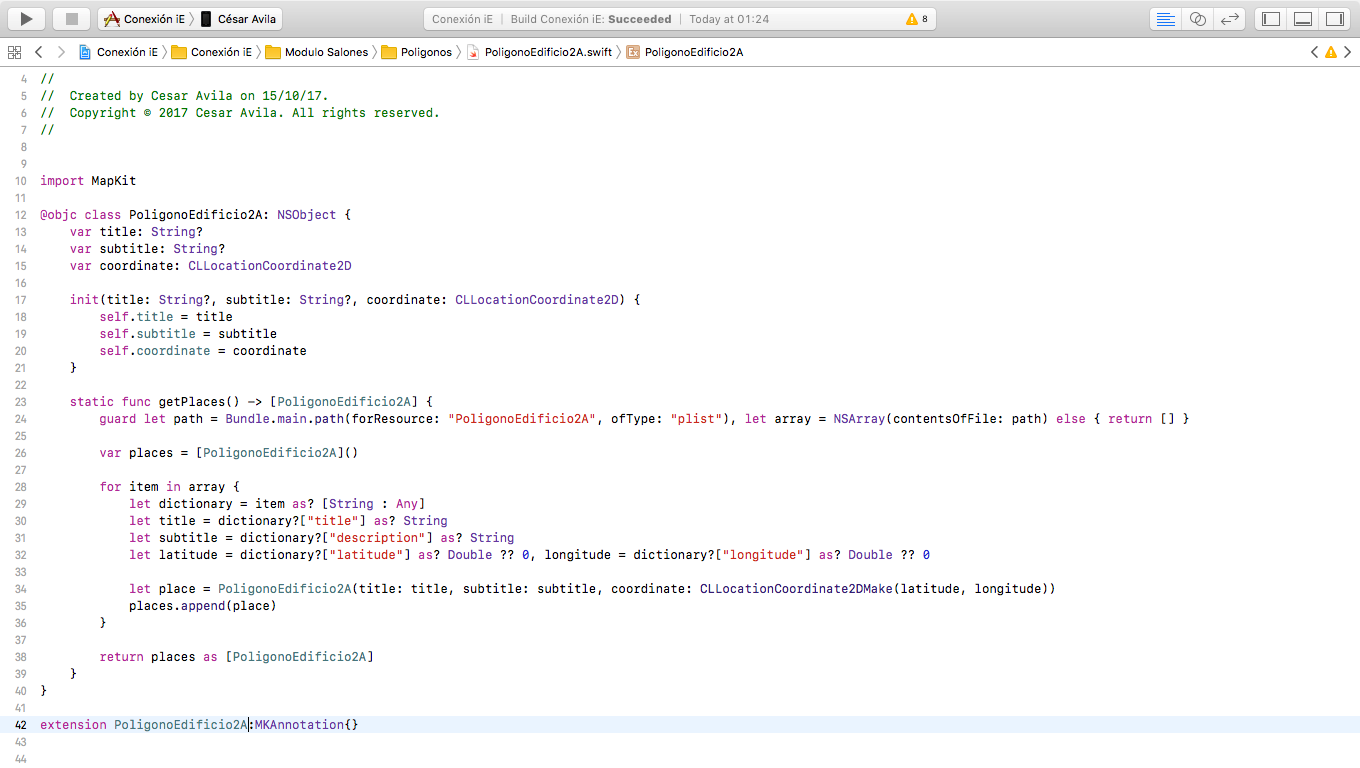
\includegraphics[width=\textwidth]{images/codigos/edificioplist}}	
		\caption{Lectura de coordenadas del Property List.}
		\label{edificioplist}
	\end{center}
\end{figure}
 \begin{figure}[h!]
	\begin{center}
		\fbox{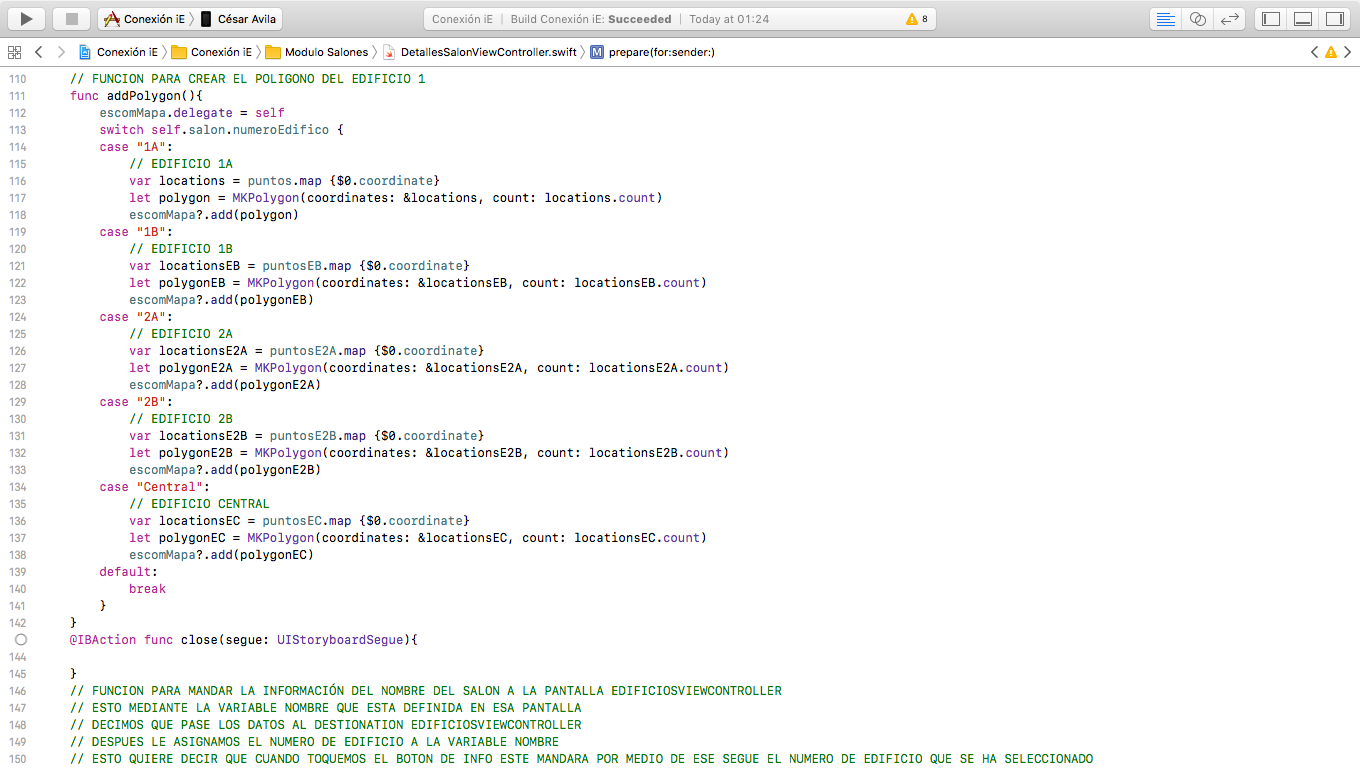
\includegraphics[width=\textwidth]{images/codigos/poligono}}	
		\caption{Creación de los Polígonos.}
		\label{poligono}
	\end{center}
\end{figure}
  \begin{figure}[h!]
 	\begin{center}
 		\fbox{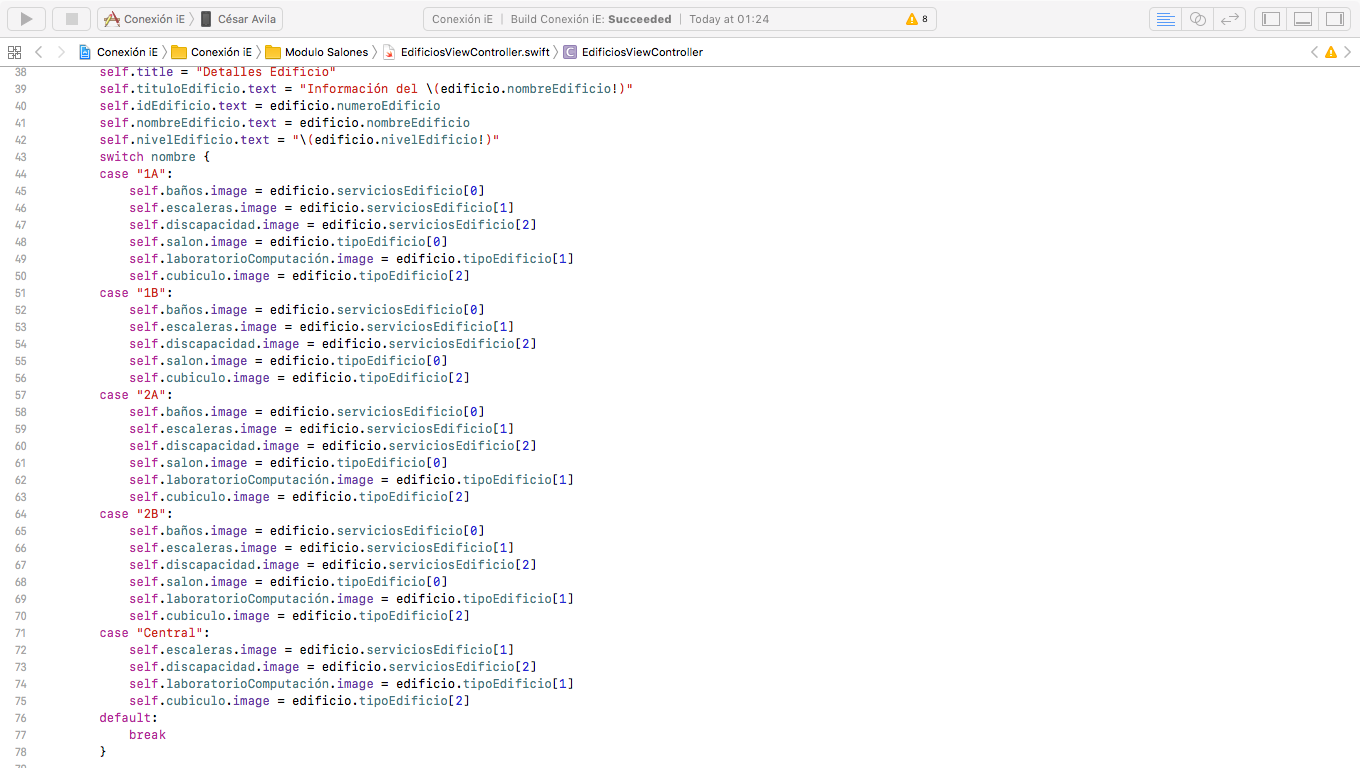
\includegraphics[width=\textwidth]{images/codigos/detallesedificio}}	
 		\caption{Clase de Detalles del Edifico.}
 		\label{detalleedificio}
 	\end{center}
 \end{figure}
 
 Teniendo como resultado las funcionales descritas anteriormente, se muestran en las figuras:
 
 \begin{figure}[h!]
 	\begin{center}
 		\fbox{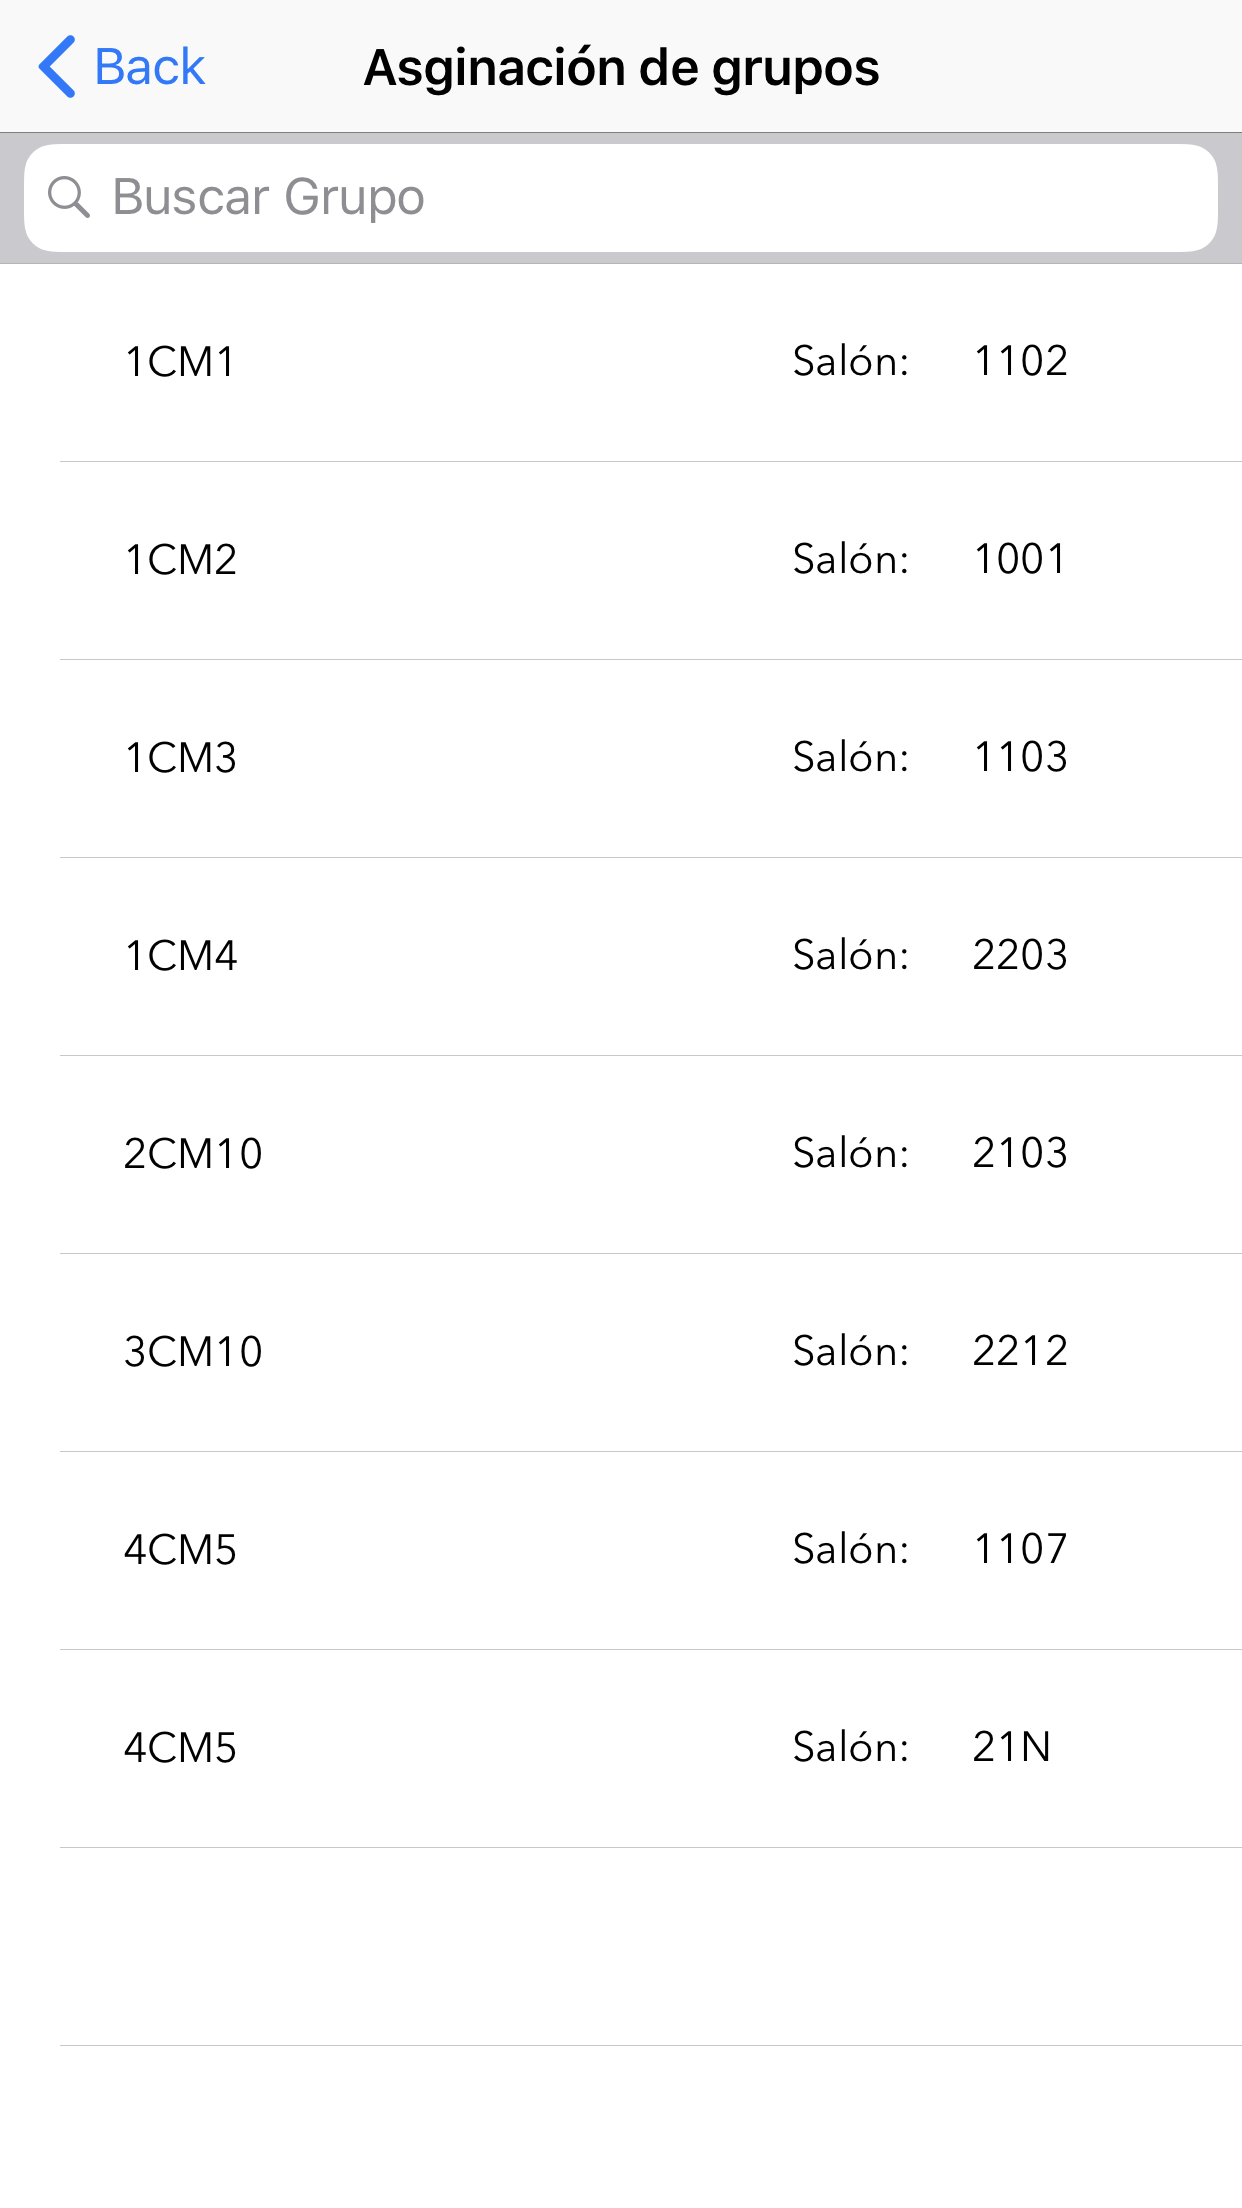
\includegraphics[width=0.3\textwidth]{images/resultados/S1}}
 		\caption{Experiencia de Profesor Seleccionado.}
 		\label{p2}
 	\end{center}
 \end{figure}
\begin{figure}[h!]
	\begin{center}
		\fbox{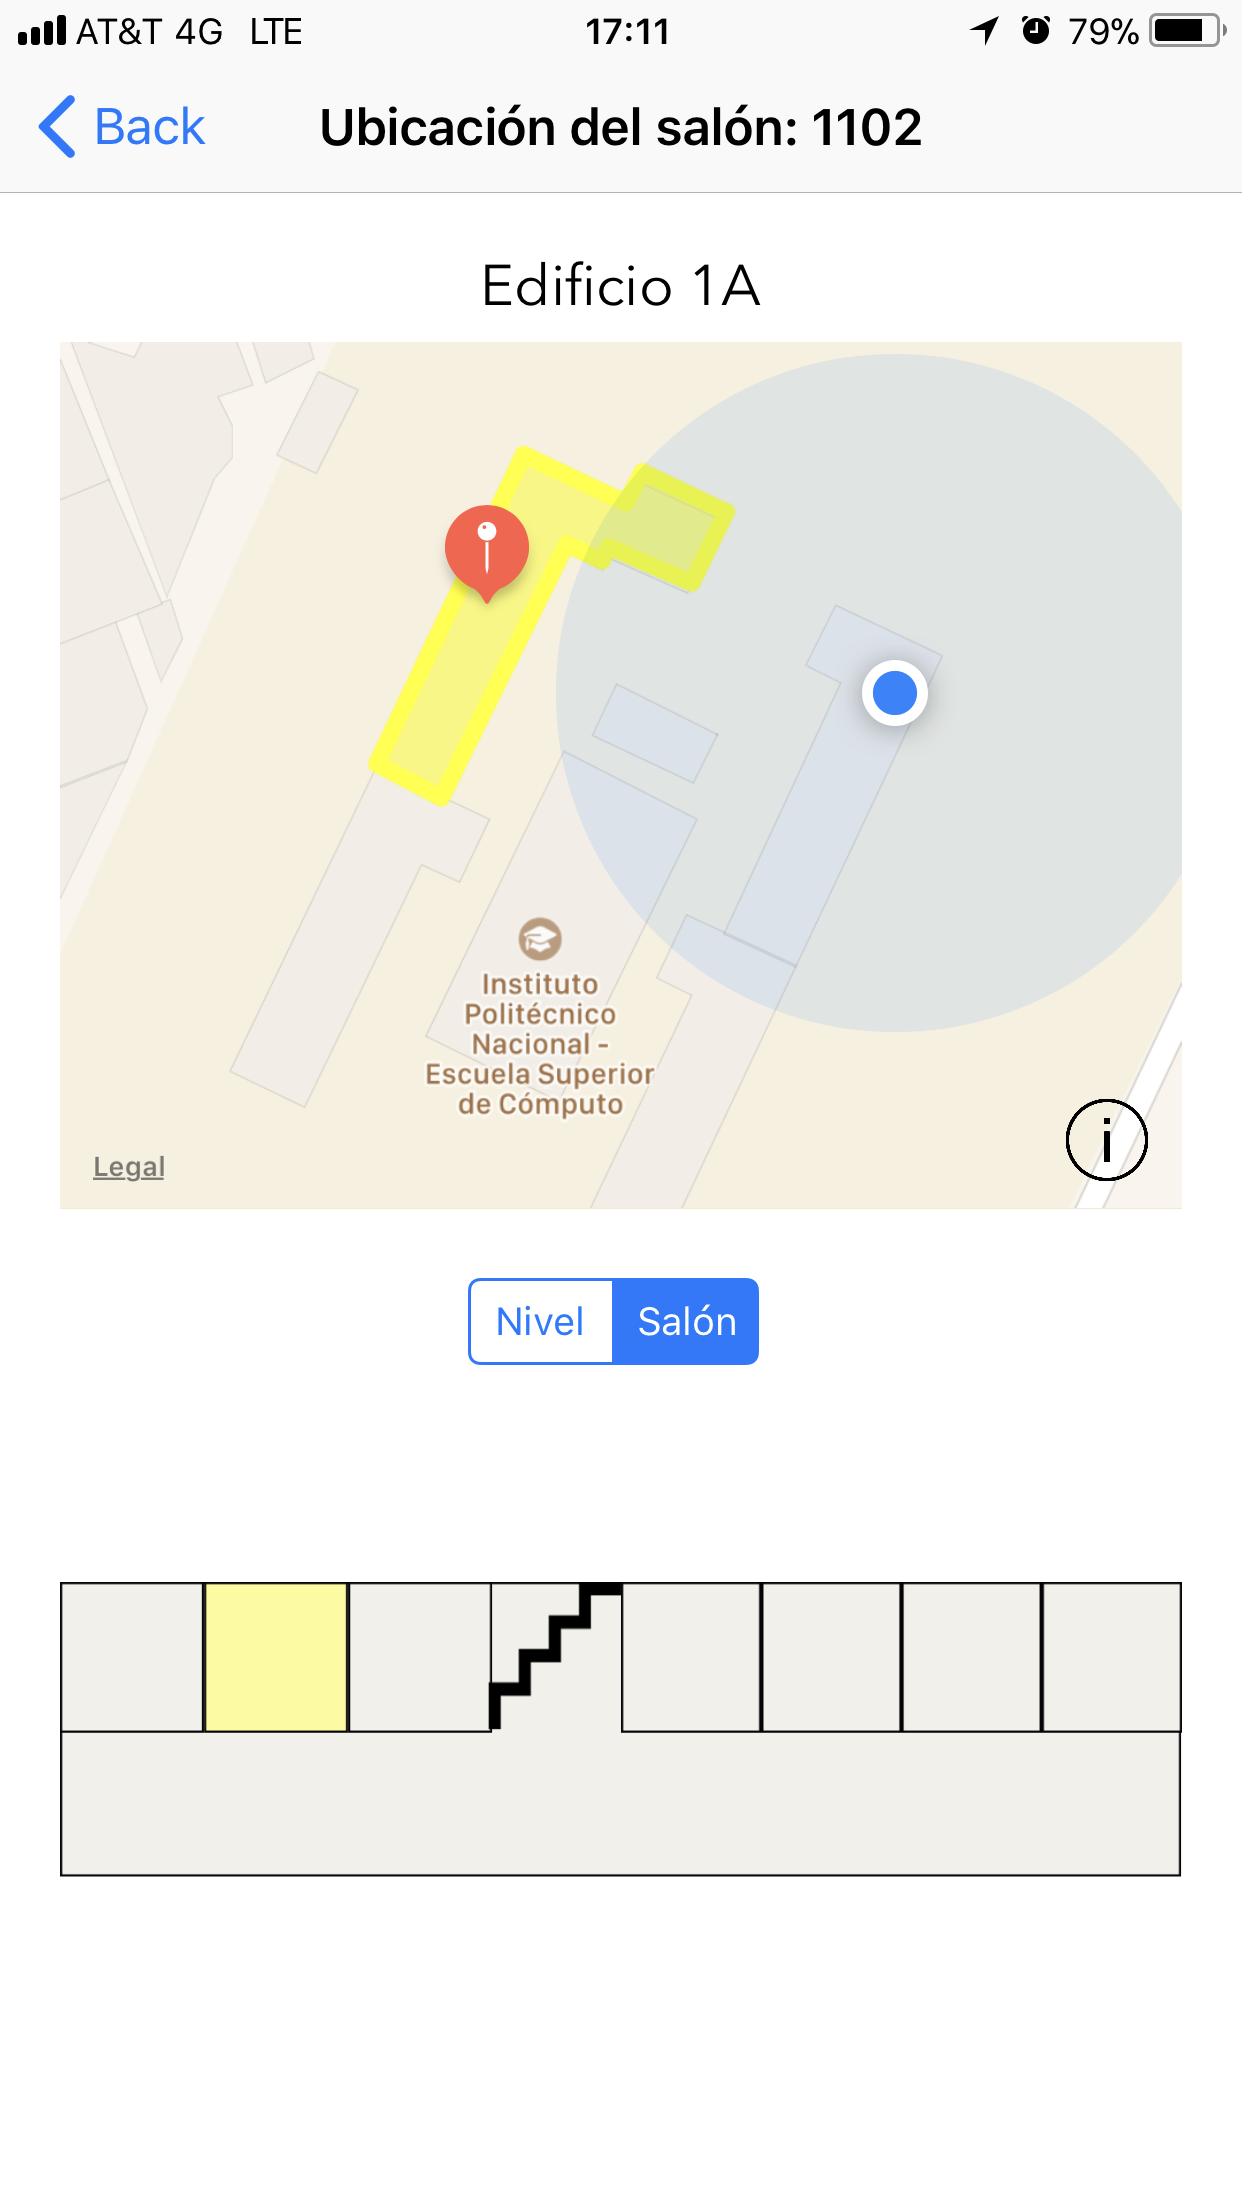
\includegraphics[width=0.3\textwidth]{images/resultados/S2}}
		\caption{Experiencia de Profesor Seleccionado.}
		\label{p2}
	\end{center}
\end{figure}
\begin{figure}[h!]
	\begin{center}
		\fbox{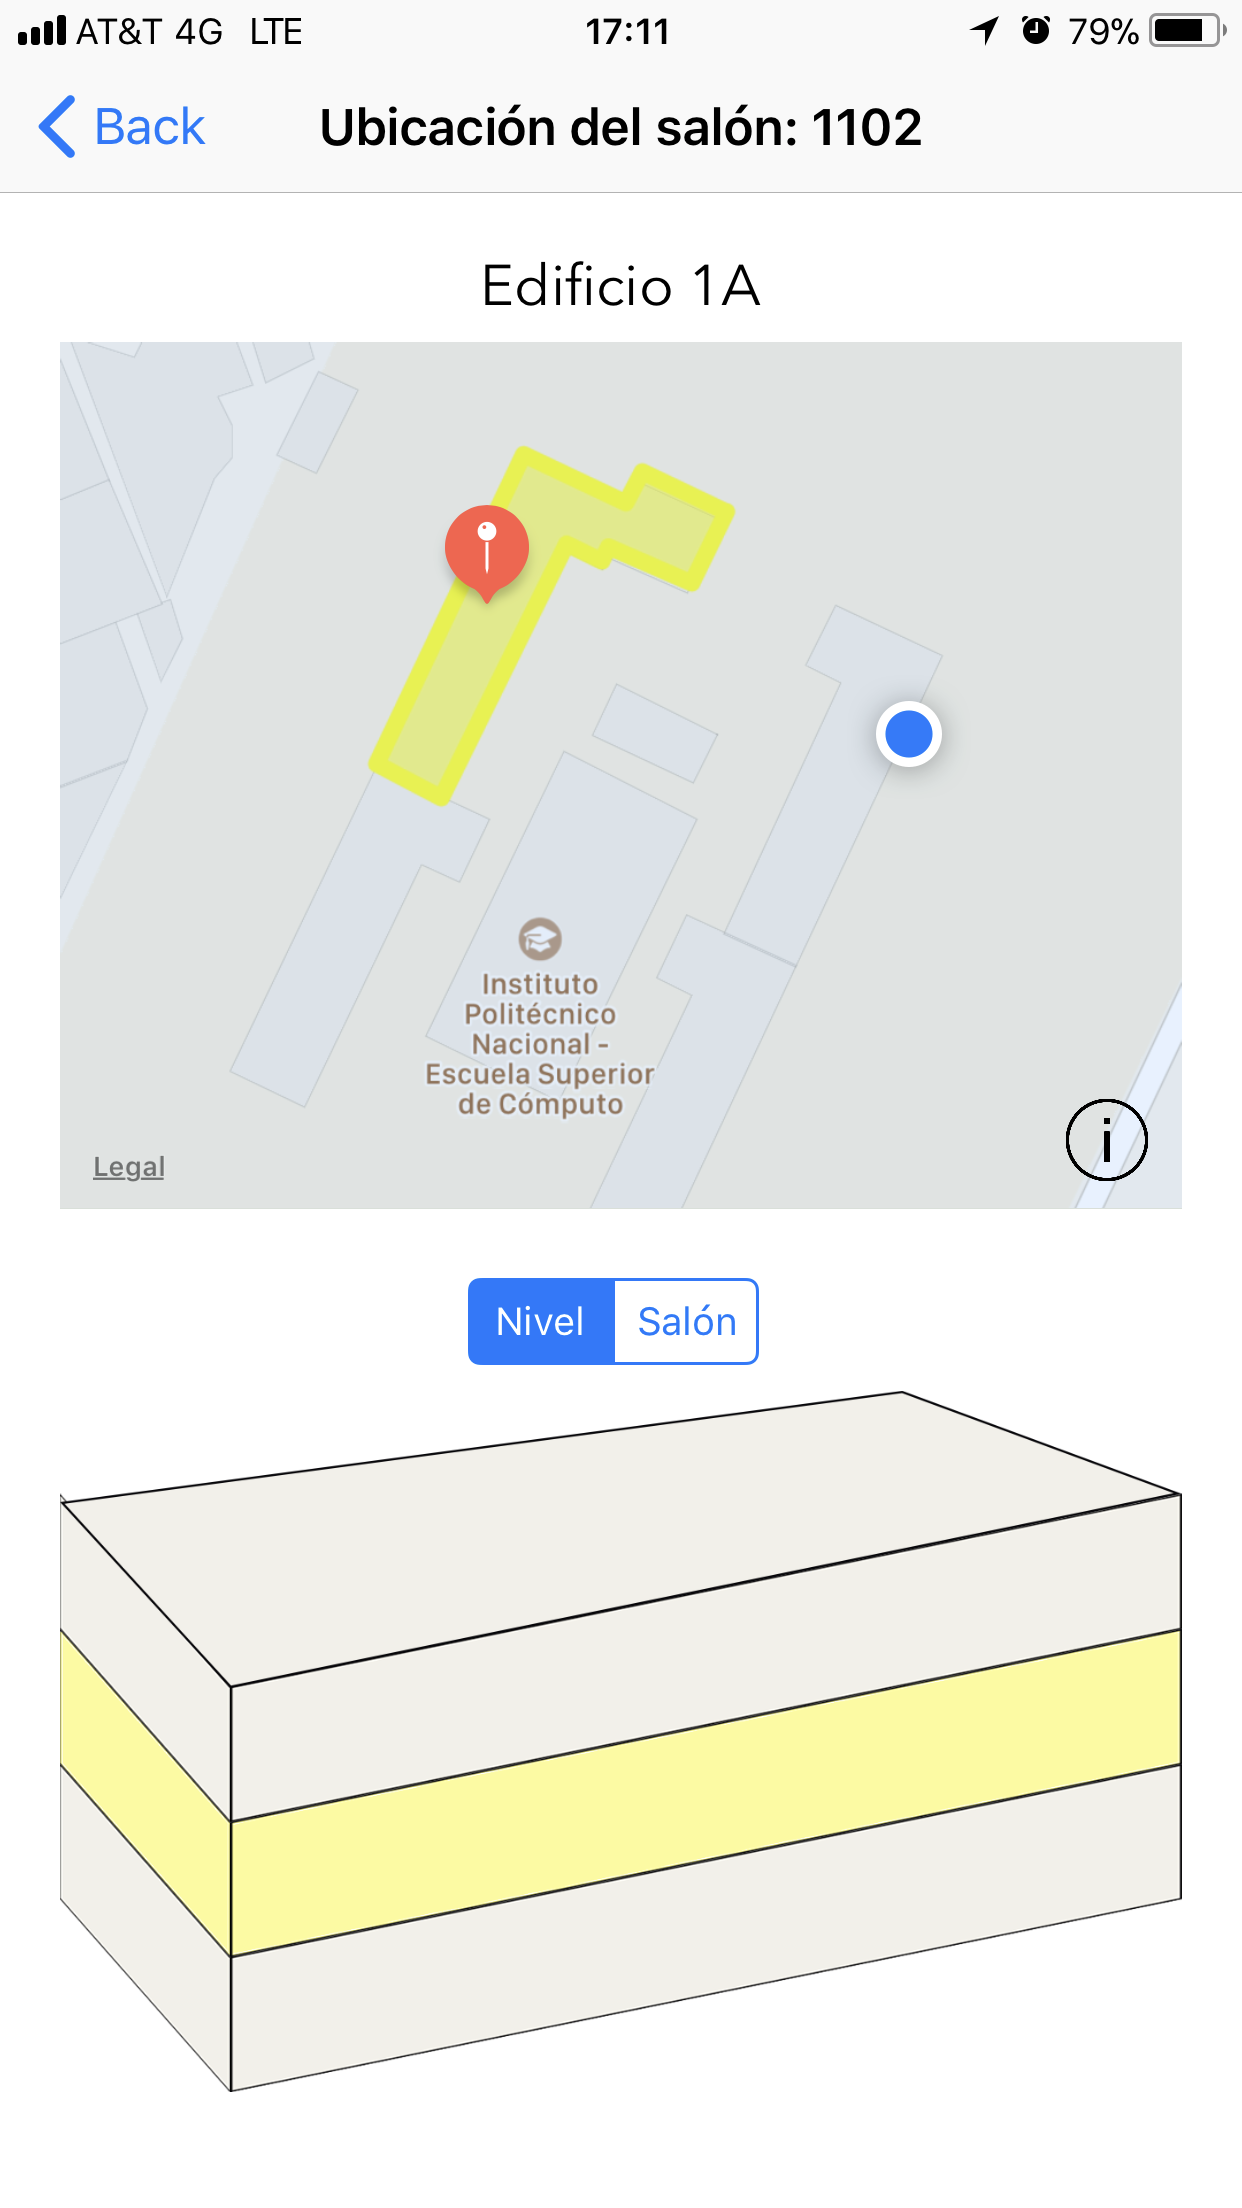
\includegraphics[width=0.3\textwidth]{images/resultados/S3}}
		\caption{Experiencia de Profesor Seleccionado.}
		\label{p2}
	\end{center}
\end{figure}
\begin{figure}[h!]
	\begin{center}
		\fbox{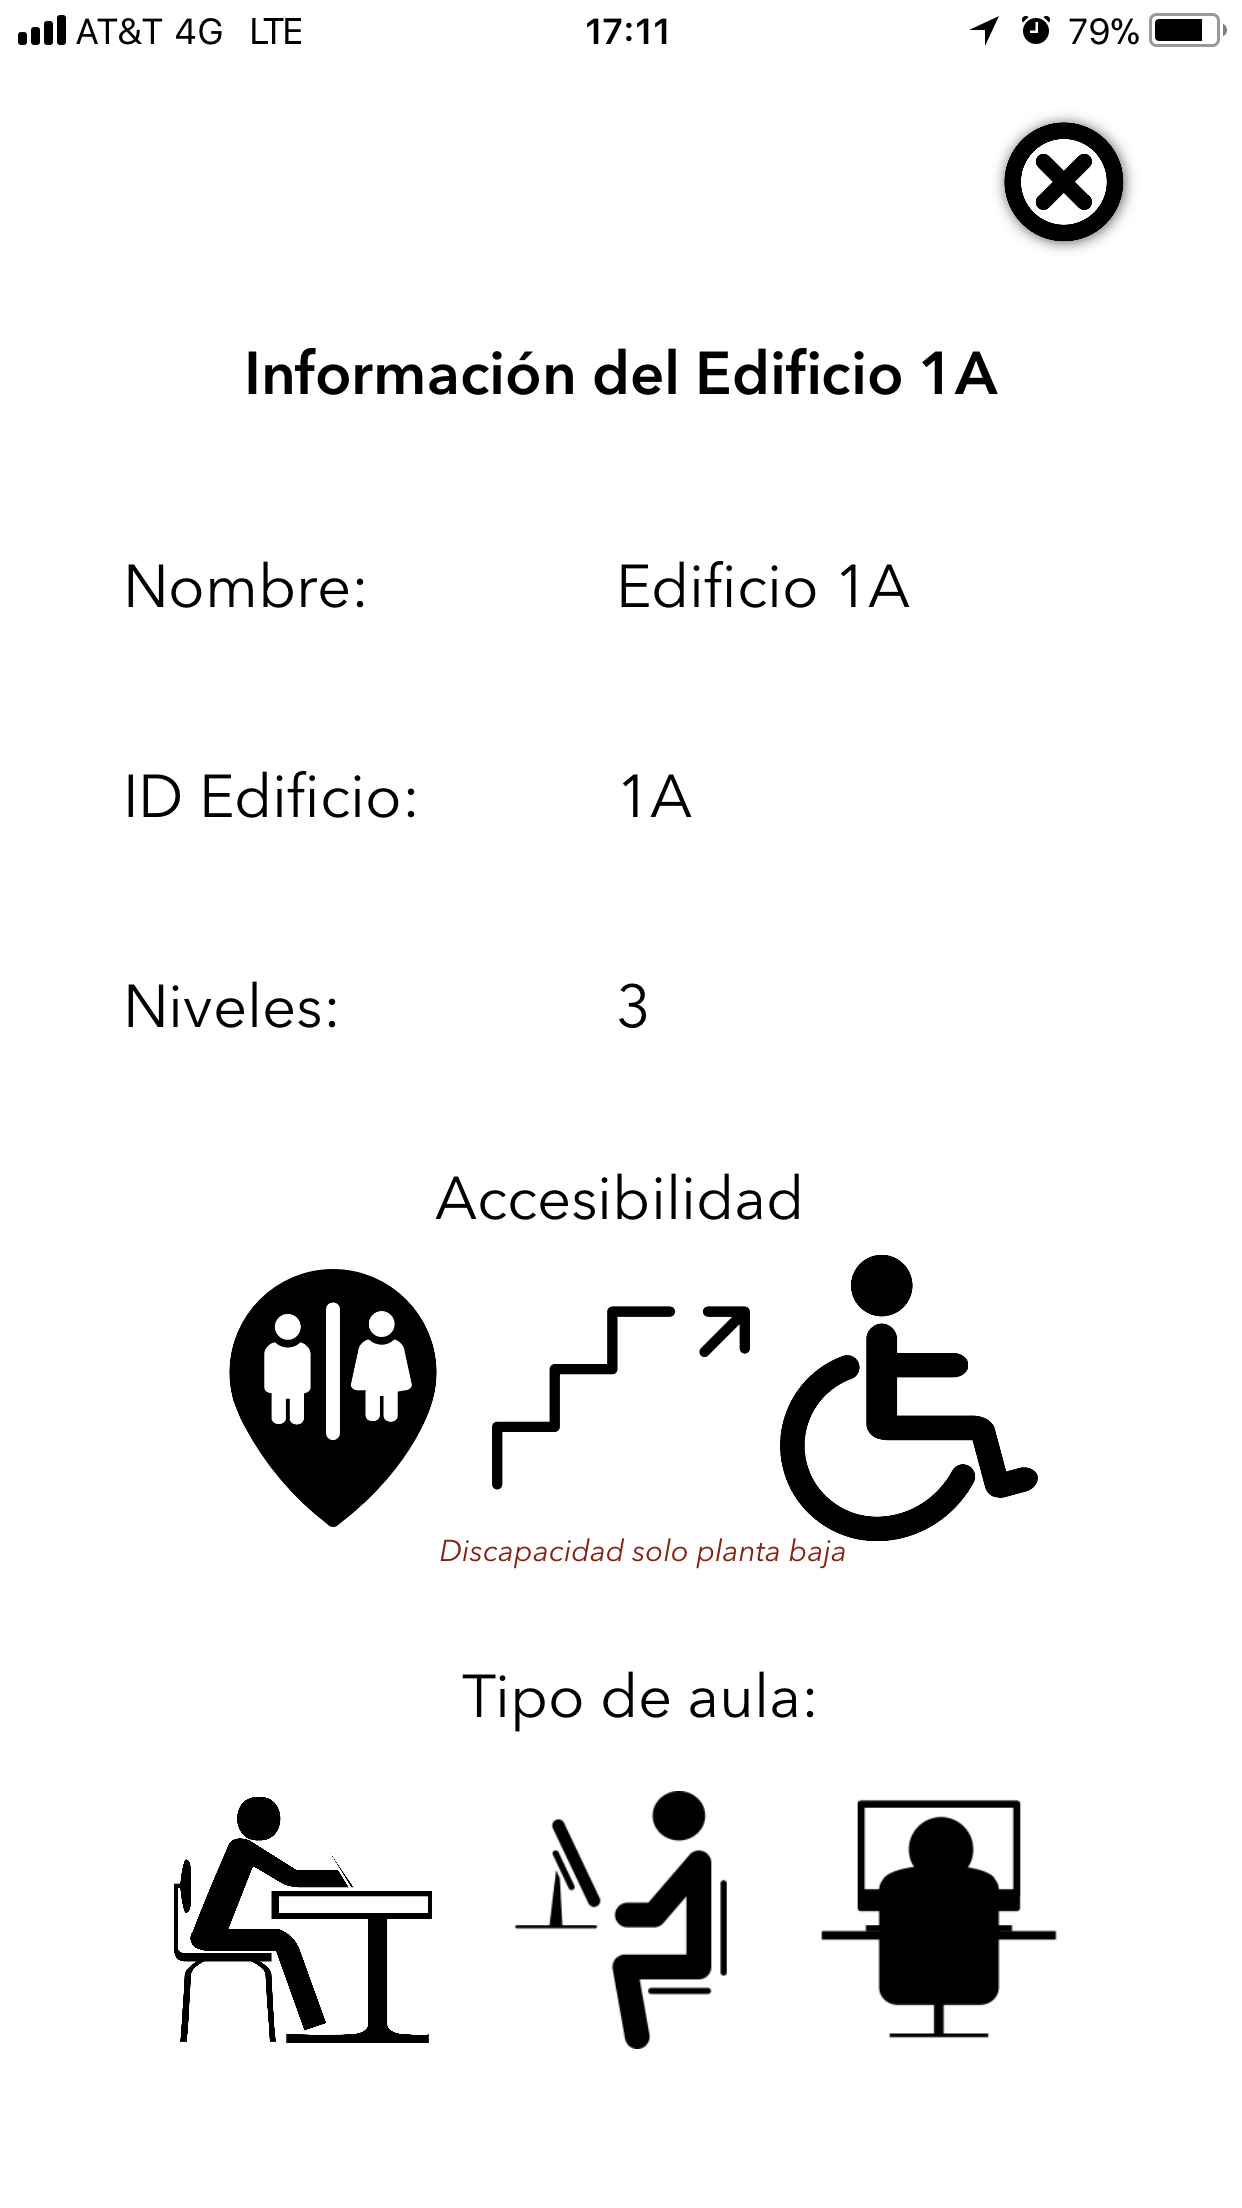
\includegraphics[width=0.3\textwidth]{images/resultados/S4}}
		\caption{Experiencia de Profesor Seleccionado.}
		\label{p2}
	\end{center}
\end{figure}